% !TeX spellcheck = en_US
\section{Problem 4}

In this problem, we are asked to write a program that implements backpropagation algorithm for an $1 - S^1 - 1$ network with $S^1=\left\{2,8,12\right\}$, as shown in figure~\ref{fig:prob4_nns}.

The first layer has $logsig$ as activation function and the output layer has $ReLU$ as activation function. Also, every weight and bias is initialized to a uniformly random number in $\left(-0.5, 0.5\right)$.
All of the above are done in order to train our network to approximate the following function:
\[
g(p) = 1 + e^{p\left(\dfrac{3\pi}{8}\right)}, \qquad p \in \left[-2,2\right]
\]

This means that, during training, we have to train the network for multiple input data (\textit{specifically, for all input data}).

\begin{figure}[H]
	\centering
	\begin{subfigure}{0.47\textwidth}
		\centering
		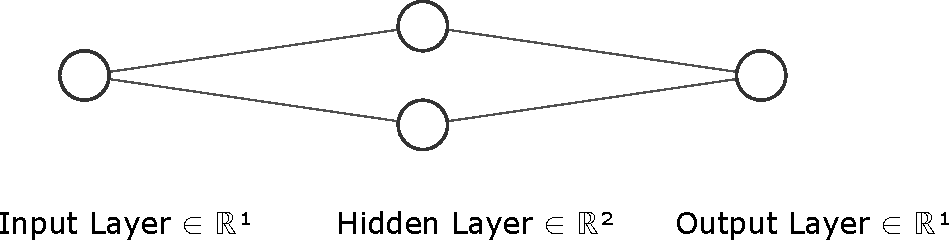
\includegraphics[width=0.9\textwidth]{../Problem 4/nn_1_2_1.pdf}
		\caption{$S^1=2$}
	\end{subfigure}
	\begin{subfigure}{0.47\textwidth}
		\centering
		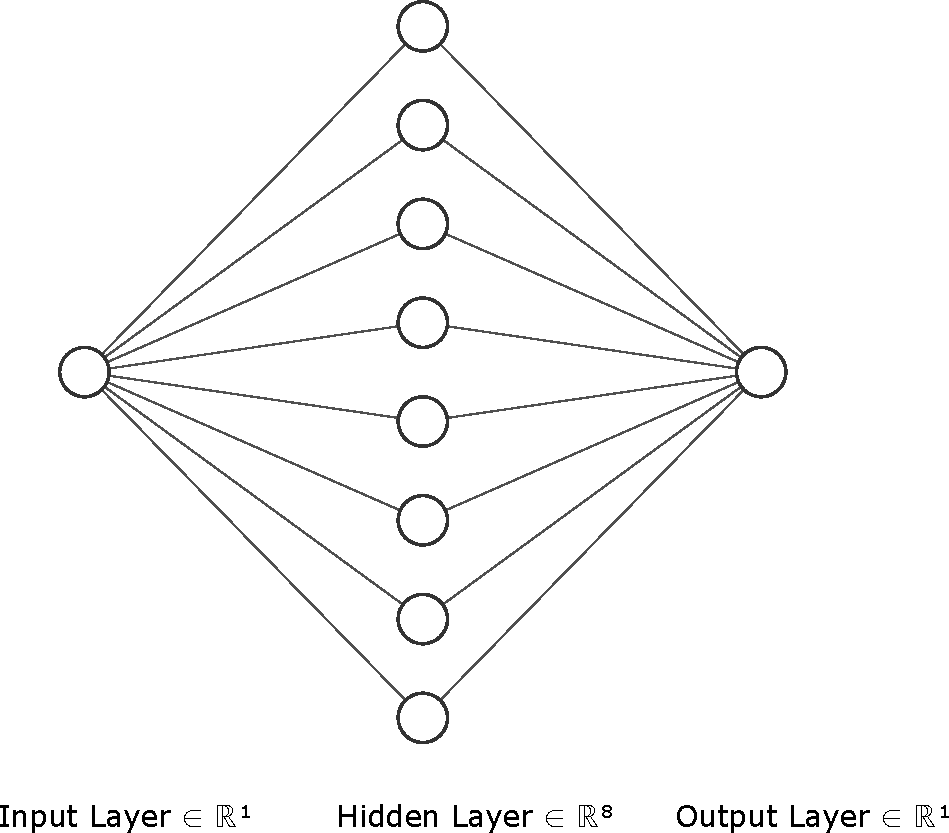
\includegraphics[width=0.9\textwidth]{../Problem 4/nn_1_8_1.pdf}
		\caption{$S^1=8$}
	\end{subfigure}
	\begin{subfigure}{0.47\textwidth}
		\centering
		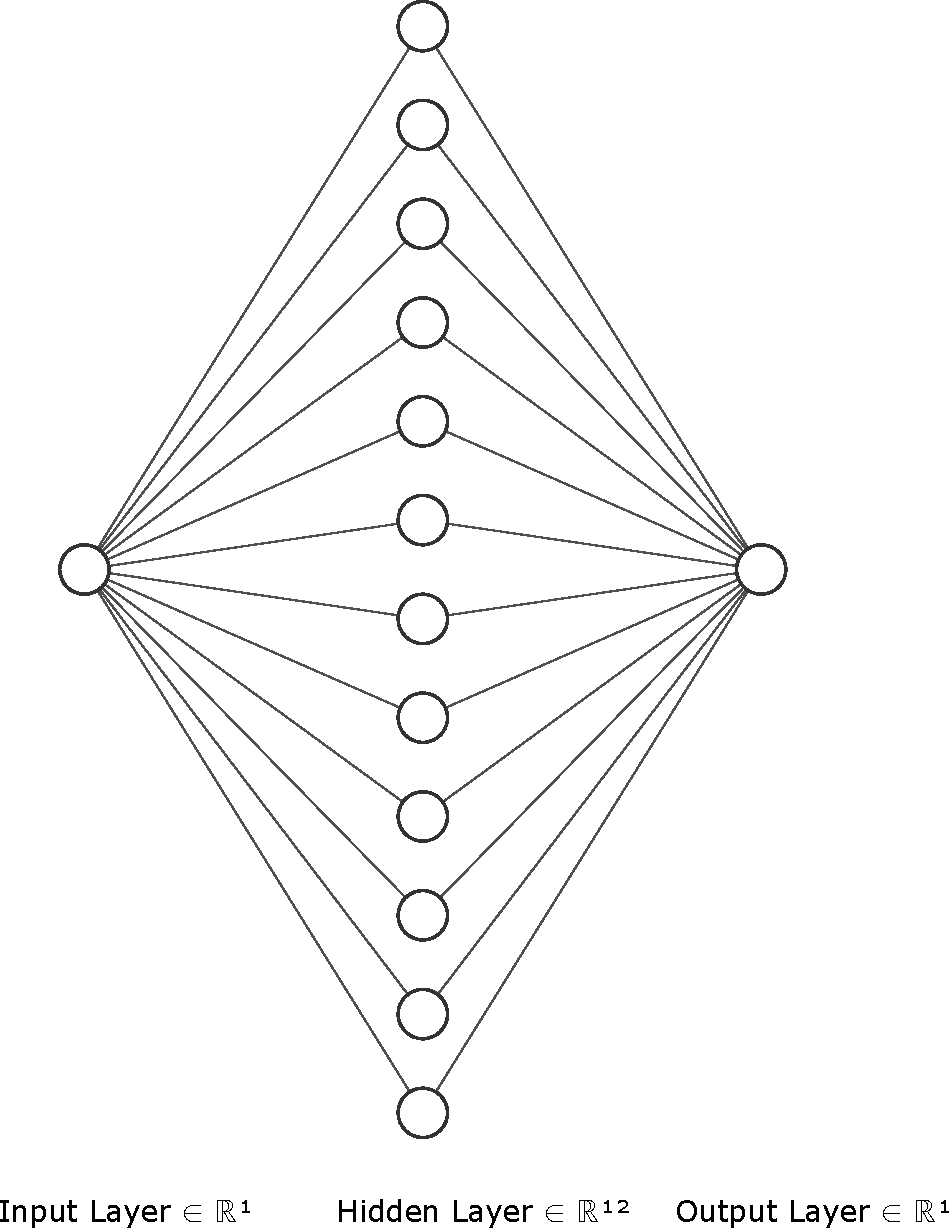
\includegraphics[width=\textwidth]{../Problem 4/nn_1_12_1.pdf}
		\caption{$S^1=12$}
	\end{subfigure}
	\caption{All the neural networks in this problem.}
	\label{fig:prob4_nns}
\end{figure}

We chose to write this program in MATLAB, despite the majority of these problems being written in Python. This ensures that we are going to use matrix operations for initialization of all weights and biases, as we're mostly familiar with this language.
The file \say{\textit{backpropagation.m}} contains all of the necessary code.\\

In order to see what difference $S$ and learning rate does to our network, we defined the following learning rates $\left[0.1, 0.01, 0.03, 0.001\right]$ and generated the network's output and error throughout training.

%From the first view, we can see in figure~\ref{fig:prob4_1_2_1_failed_attempt} that 
From the very first run ($S=2,\ \alpha=0.001$), we can see in figure~\ref{fig:prob4_1_2_1_failed_attempt} that the back-propagation algorithm didn't converge at all, keeping the error to a constant value throughout the epochs.

\begin{figure}[htpb]
	\centering
	\begin{subfigure}{0.47\textwidth}
		\centering
		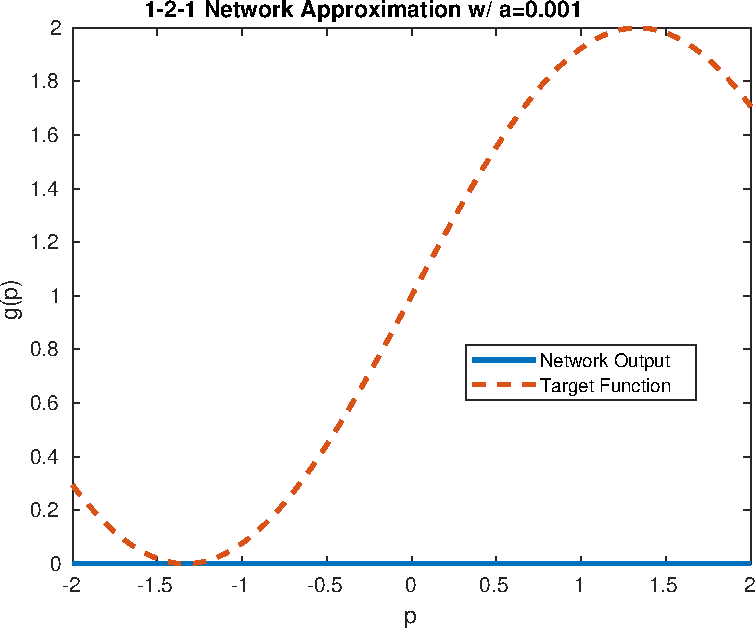
\includegraphics[width=\textwidth]{../Problem 4/1_2_1_failed_approximation.pdf}
		\caption{Approximation of input signal}
	\end{subfigure}
	\begin{subfigure}{0.47\textwidth}
		\centering
		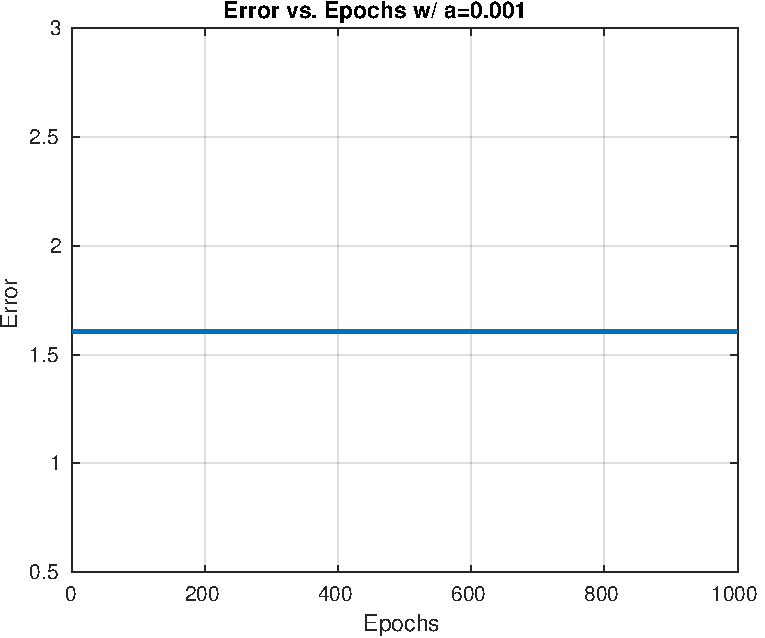
\includegraphics[width=\textwidth]{../Problem 4/1_2_1_failed_approximation_error.pdf}
		\caption{Error over iterations}
	\end{subfigure}
	\caption{A failed attempt of approximating the input signal. \\ The reason this approximation failed derives from the uniformly random initial guess for the weights and biases.}
	\label{fig:prob4_1_2_1_failed_attempt}
\end{figure}

After taking a closer look in the code, we can see the point of failure of the algorithm. Below, there's a snippet of the code that calculates the back-propagation.

\begin{lstlisting}[language=matlab]
	e = g(i) - a2;
	s2 = -2*e*relu_derivative(n2);
	s1 = logsig_derivative(n1) .* W2' .* s2;
\end{lstlisting}

We can see that both sensitivities depends on \verb*|s2|, a value that itself depends on $ReLU$'s derivative, which has the following expression:
\[
\dfrac{d\ ReLU\left(x\right)}{dx} = \left\{ 
\begin{array}{cc}
	1, & x >0\\
	0, & x<0
\end{array}
\right.
\]

So, if $n^2$ is a negative number, $ReLU$'s derivative will be $0$, zeroing out both sensitivities and effectively stalling the back-propagation algorithm. Thus, in order for the algorithm to make progress, $n^2$ \underline{must} be a positive number.
So, we altered the code and added an if statement that stops the algorithm if variable \verb*|s2=0| and \verb*|epoch=1|. In this way, we stop unnecessary calculations and start over, hopping that the random initialization of the weights and biases will not give us another configuration like the one above. \\

After describing the unexpected issue and its solution, we can focus on the real matter which is the accuracy of the algorithm across different learning rates and number of neurons in the first hidden layer. Figures~\ref{fig:prob4_1-2-1_error_output}, \ref{fig:prob4_1-8-1_error_output} and \ref{fig:prob4_1-12-1_error_output} contains every figure for every $S^1$ and learning rate $\alpha$.

\begin{figure}[htpb]
	\centering
	\begin{subfigure}{0.47\textwidth}
		\centering
		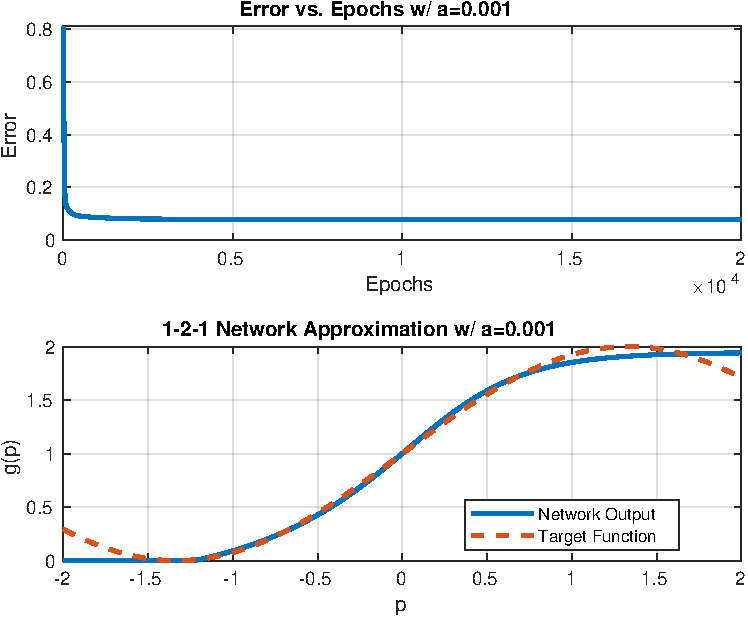
\includegraphics[width=\textwidth]{../Problem 4/nn_images/1-2-1_NN_a=0.001.pdf}
		\caption{}
	\end{subfigure}
	\hfill
	\begin{subfigure}{0.47\textwidth}
		\centering
		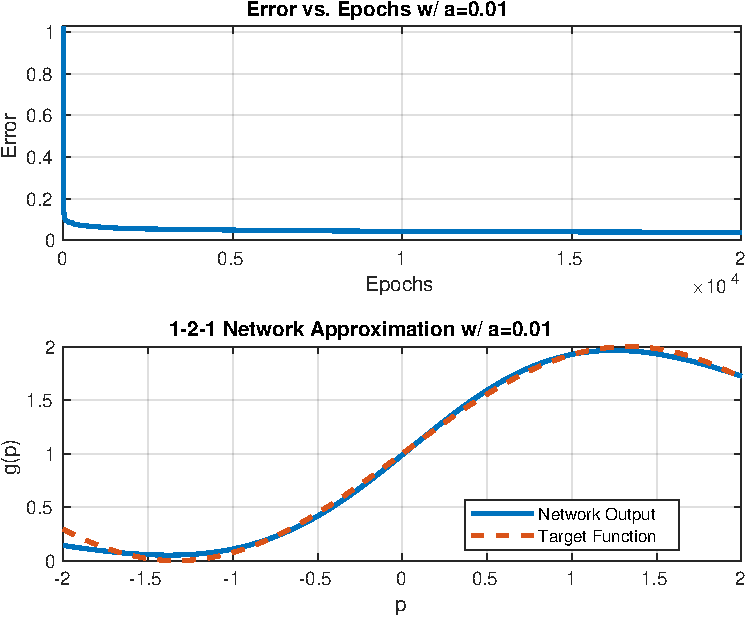
\includegraphics[width=\textwidth]{../Problem 4/nn_images/1-2-1_NN_a=0.01.pdf}
		\caption{}
	\end{subfigure}\\
	\vspace{1cm}
	\begin{subfigure}{0.47\textwidth}
		\centering
		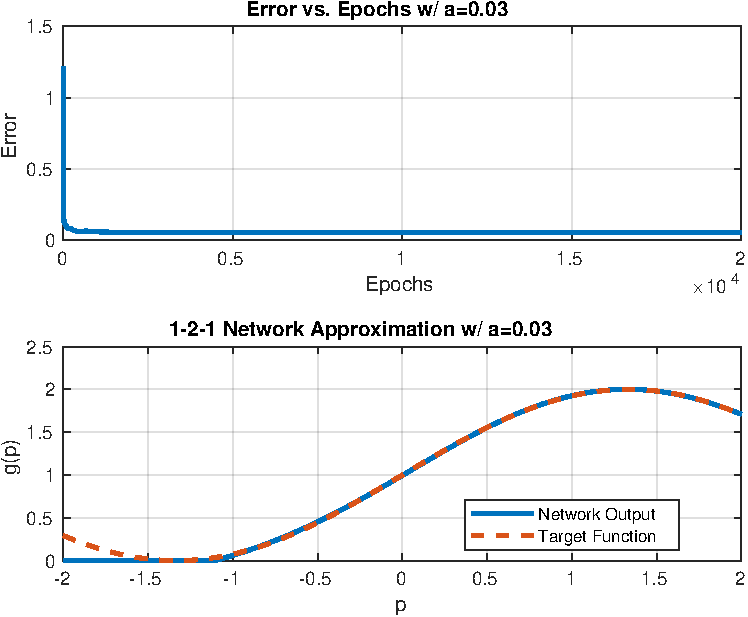
\includegraphics[width=\textwidth]{../Problem 4/nn_images/1-2-1_NN_a=0.03.pdf}
		\caption{}
	\end{subfigure}
	\hfill
	\begin{subfigure}{0.47\textwidth}
		\centering
		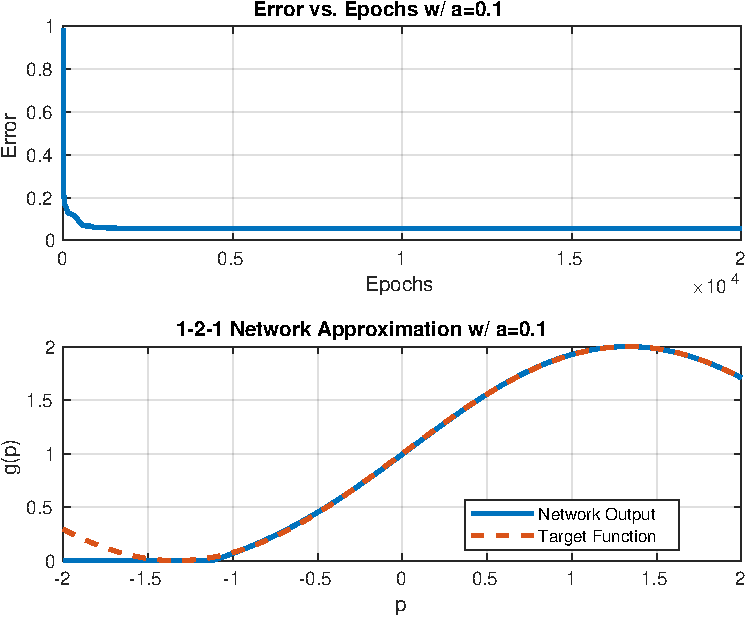
\includegraphics[width=\textwidth]{../Problem 4/nn_images/1-2-1_NN_a=0.1.pdf}
		\caption{}
	\end{subfigure}
	\caption{Error over iterations and approximation, $S^1=2$}
	\label{fig:prob4_1-2-1_error_output}
\end{figure}

\begin{figure}[htpb]
	\centering
	\begin{subfigure}{0.47\textwidth}
		\centering
		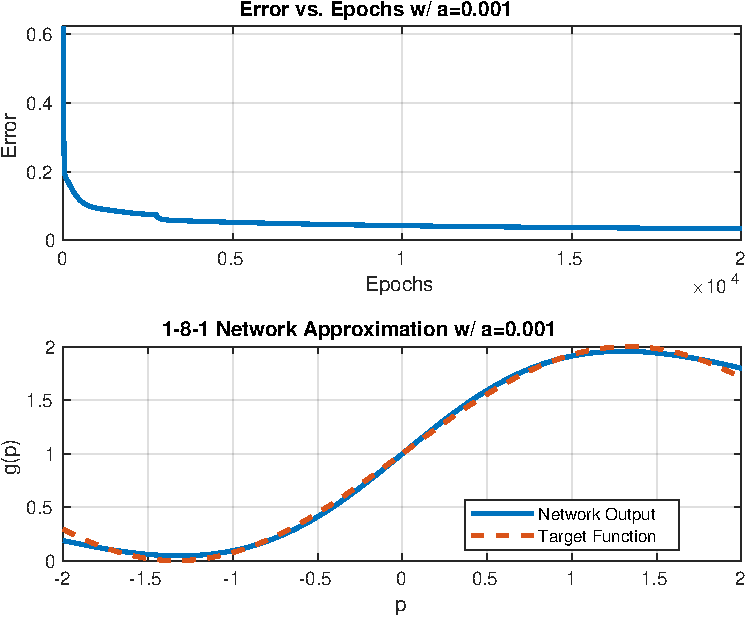
\includegraphics[width=\textwidth]{../Problem 4/nn_images/1-8-1_NN_a=0.001.pdf}
		\caption{}
	\end{subfigure}
	\hfill
	\begin{subfigure}{0.47\textwidth}
		\centering
		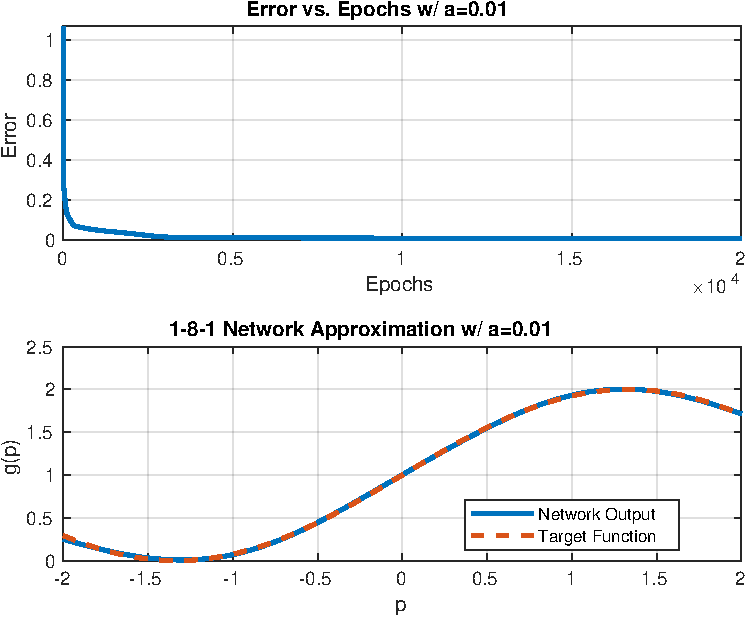
\includegraphics[width=\textwidth]{../Problem 4/nn_images/1-8-1_NN_a=0.01.pdf}
		\caption{}
	\end{subfigure}\\
	\vspace{1cm}
	\begin{subfigure}{0.47\textwidth}
		\centering
		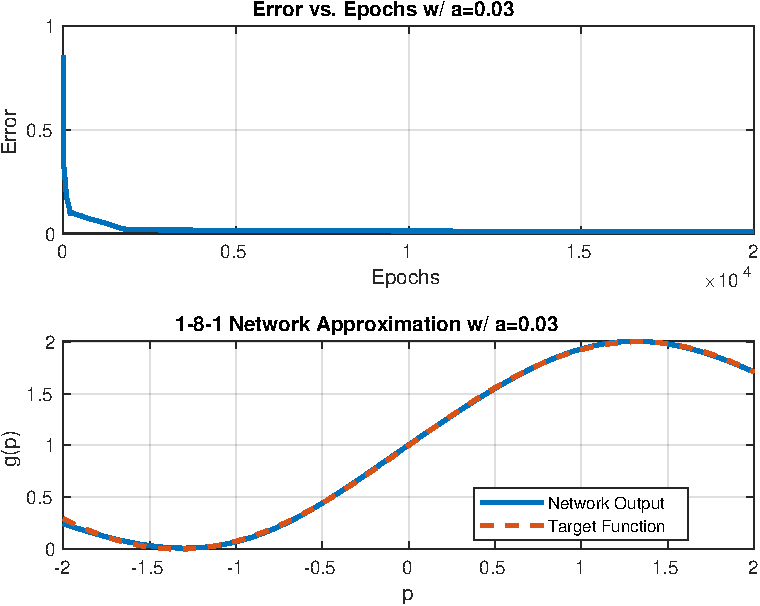
\includegraphics[width=\textwidth]{../Problem 4/nn_images/1-8-1_NN_a=0.03.pdf}
		\caption{}
	\end{subfigure}
	\hfill
	\begin{subfigure}{0.47\textwidth}
		\centering
		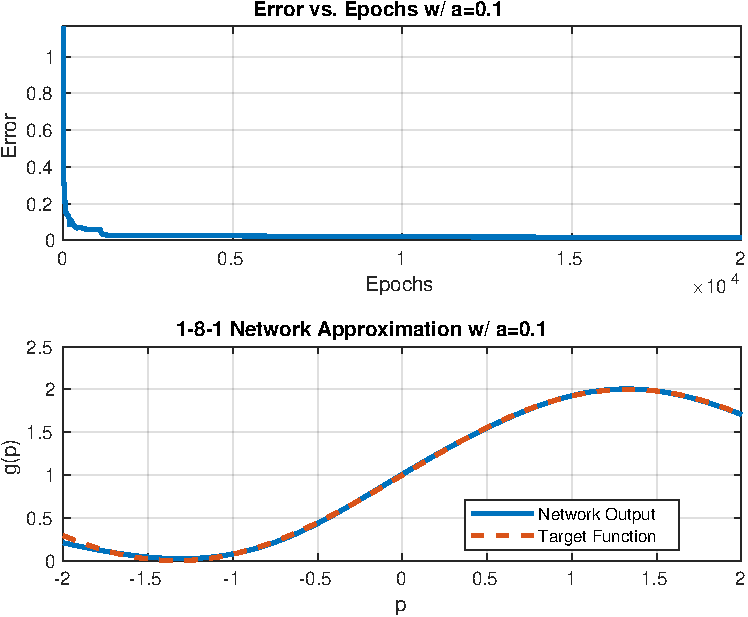
\includegraphics[width=\textwidth]{../Problem 4/nn_images/1-8-1_NN_a=0.1.pdf}
		\caption{}
	\end{subfigure}
	\caption{Error over iterations and approximation, $S^1=8$}
	\label{fig:prob4_1-8-1_error_output}
\end{figure}

\begin{figure}[htpb]
	\centering
	\begin{subfigure}{0.47\textwidth}
		\centering
		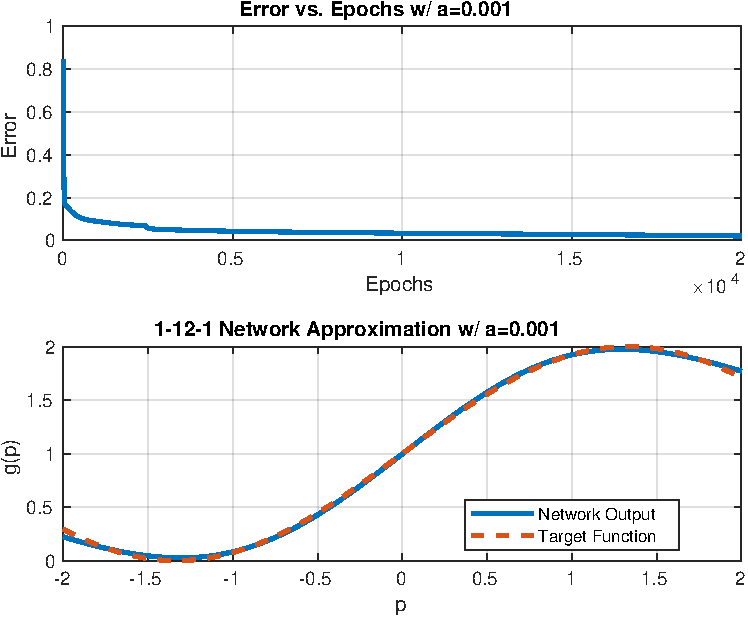
\includegraphics[width=\textwidth]{../Problem 4/nn_images/1-12-1_NN_a=0.001.pdf}
		\caption{}
	\end{subfigure}
	\hfill
	\begin{subfigure}{0.47\textwidth}
		\centering
		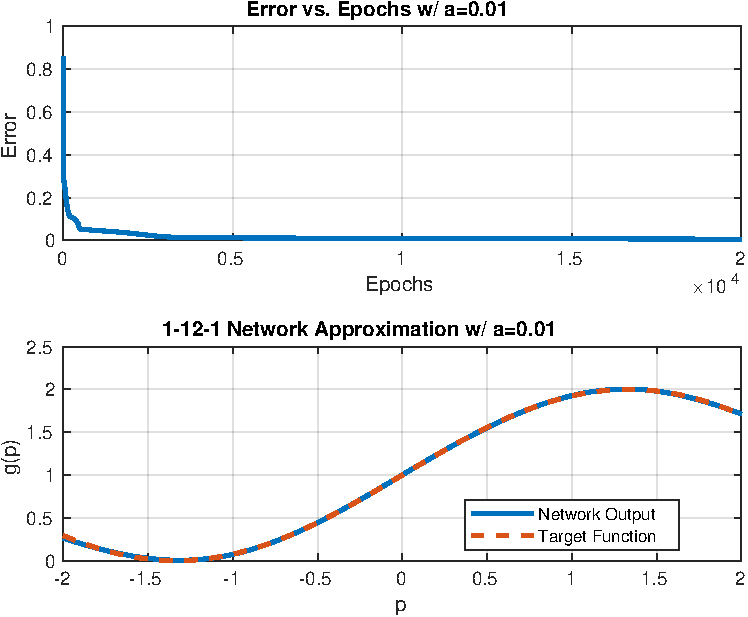
\includegraphics[width=\textwidth]{../Problem 4/nn_images/1-12-1_NN_a=0.01.pdf}
		\caption{}
	\end{subfigure}\\
	\vspace{1cm}
	\begin{subfigure}{0.47\textwidth}
		\centering
		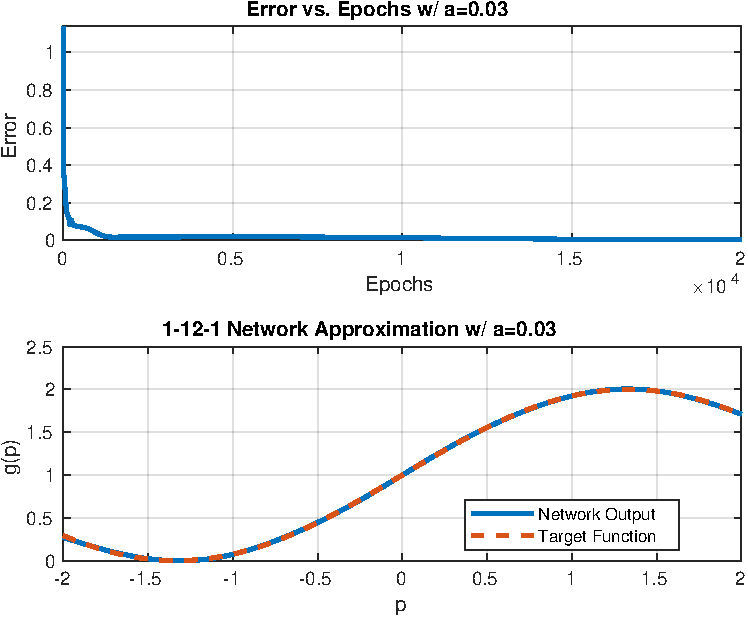
\includegraphics[width=\textwidth]{../Problem 4/nn_images/1-12-1_NN_a=0.03.pdf}
		\caption{}
	\end{subfigure}
	\hfill
	\begin{subfigure}{0.47\textwidth}
		\centering
		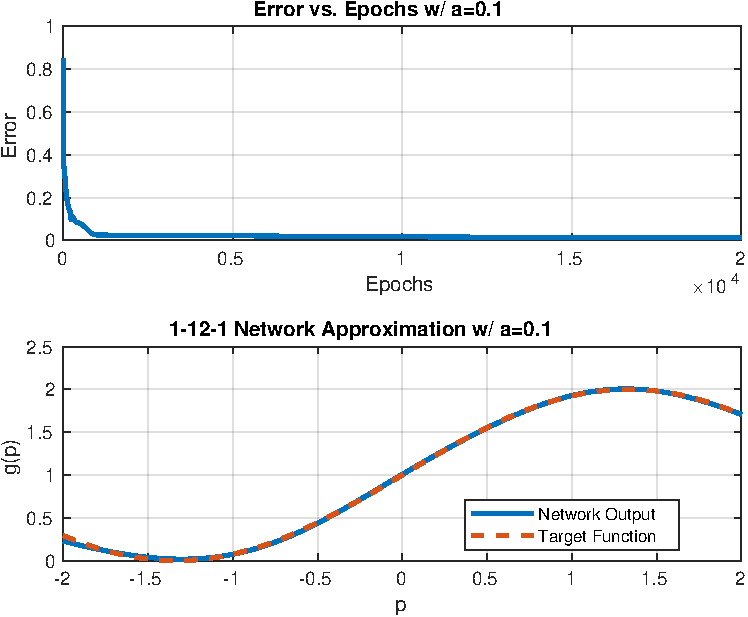
\includegraphics[width=\textwidth]{../Problem 4/nn_images/1-12-1_NN_a=0.1.pdf}
		\caption{}
	\end{subfigure}
	\caption{Error over iterations and approximation, $S^1=12$}
	\label{fig:prob4_1-12-1_error_output}
\end{figure}

The error plotted in every figure is the mean square approximation error described below:
\begin{lstlisting}[language=matlab]
	err = abs(a2_error' - g).^2;
	err_plt(epoch) = sqrt(mean(err));
\end{lstlisting}

As far as the learning rate $\alpha$ is concerned, we can observe that decreasing $\alpha$ results in a smoother but slower convergence. This indicates a more stable learning but requires a lot more iterations to achieve optimal accuracy.
On the other hand, higher $\alpha$ speed up convergence initially, but the end result is not great when comparing to smaller $\alpha$ values. Looking at the approximated functions, we can see that for $\alpha=0.1$ (\textit{\small which is a relatively big value}) there's a big approximation error for every $S^1$, thus accuracy is compromised.

We tried increasing $\alpha$ beyond $0.1$ but as it turned out, the algorithm failed each time either from the start or later. Regardless, we couldn't get any remarkable results for the report.\\

Moving on to the capacity of the hidden layer, there's a big change in the accuracy of the neural network as it's increased.
Looking at figure~\ref{fig:prob4_1-2-1_error_output}, we can see that there's a fairly large area at the start and end of $p$, where the approximation is way off the input signal.
As $S^1$ increases, the function's approximation on the areas described above is getting smaller as seen in figures~\ref{fig:prob4_1-8-1_error_output} and \ref{fig:prob4_1-12-1_error_output}. Particularly, in the latter the error drops very low for $\alpha=0.03$ and the approximation is almost the same as the original signal.
Also, this can be seen in the \say{Error vs Epochs} plot where the error drops very low. \\


In conclusion, our experiments reveal a subtle relationship between the learning rate, $\alpha$, and the capacity of the neural network, as defined by the number of hidden neurons, $S^1$. A lower $\alpha$ ensures stable and smooth convergence, albeit at the cost of increased iterations for optimal accuracy. Conversely, a higher $\alpha$ expedites convergence but at the expense of accuracy, particularly evident at $\alpha=0.1$ where the approximation error significantly increases across all $S^1$ values. Furthermore, our attempts to increase $\alpha$ beyond 0.1 resulted in algorithmic failure, underscoring the delicate balance required in tuning $\alpha$. On the capacity front, enhancing $S^1$ markedly improves the neural network's accuracy, particularly for complex function approximations as the neural network can process much more information. This is demonstrated through improved approximation closeness to the original signal with increased $S^1$, highlighting the critical role of neural network capacity in achieving high-fidelity approximations.